\usetikzlibrary{arrows.meta,positioning,calc}

\definecolor{paperdiagblue}{RGB}{230,240,252}
\definecolor{paperdiaggreen}{RGB}{236,245,230}
\definecolor{paperdiagbeige}{RGB}{244,239,230}
\definecolor{paperdiagrose}{RGB}{250,240,236}
\definecolor{paperdiagviolet}{RGB}{244,241,251}
\definecolor{paperdiaggray}{RGB}{242,242,242}
\definecolor{paperdiagdark}{RGB}{55,55,55}

\tikzset{
  paper box/.style={
    draw=paperdiagdark,
    rounded corners=2pt,
    line width=0.8pt,
    inner sep=3pt,
    align=left,
    font=\small,
  },
  paper arrow/.style={
    -{Latex[length=2.0mm,width=1.6mm]},
    line width=0.9pt,
    draw=paperdiagdark,
  },
}

\newcommand{\PaperFrameworkOverviewDiagram}{%
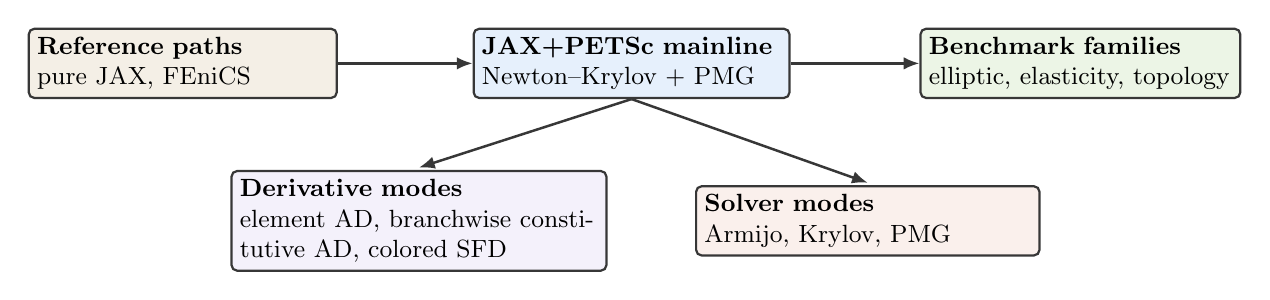
\begin{tikzpicture}[x=1cm,y=1cm]
  \node[paper box, fill=paperdiagbeige, text width=3.7cm] (ref) at (0,0)
    {\textbf{Reference paths}\\pure JAX, FEniCS};
  \node[paper box, fill=paperdiagblue, text width=3.8cm] (main) at (5.7,0)
    {\textbf{JAX+PETSc mainline}\\Newton--Krylov + PMG};
  \node[paper box, fill=paperdiaggreen, text width=3.85cm] (bench) at (11.4,0)
    {\textbf{Benchmark families}\\elliptic, elasticity, topology};
  \node[paper box, fill=paperdiagviolet, text width=4.55cm] (deriv) at (3.0,-2.0)
    {\textbf{Derivative modes}\\element AD, branchwise constitutive AD, colored SFD};
  \node[paper box, fill=paperdiagrose, text width=4.15cm] (solver) at (8.7,-2.0)
    {\textbf{Solver modes}\\Armijo, Krylov, PMG};

  \draw[paper arrow] (ref.east) -- (main.west);
  \draw[paper arrow] (main.east) -- (bench.west);
  \draw[paper arrow] (main.south) -- ($(deriv.north)+(0,0.03)$);
  \draw[paper arrow] (main.south) -- ($(solver.north)+(0,0.03)$);
\end{tikzpicture}%
}

\newcommand{\PaperDerivativePathDiagram}{%
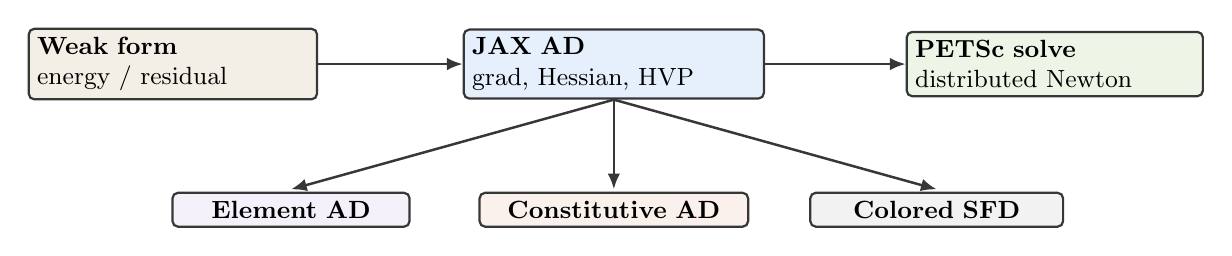
\begin{tikzpicture}[x=1cm,y=1cm]
  \node[paper box, fill=paperdiagbeige, text width=3.45cm] (weak) at (0,0)
    {\textbf{Weak form}\\energy / residual};
  \node[paper box, fill=paperdiagblue, text width=3.6cm] (jax) at (5.6,0)
    {\textbf{JAX AD}\\grad, Hessian, HVP};
  \node[paper box, fill=paperdiaggreen, text width=3.55cm] (petsc) at (11.2,0)
    {\textbf{PETSc solve}\\distributed Newton};

  \node[paper box, fill=paperdiagviolet, text width=2.8cm, align=center] (elem) at (1.5,-1.85)
    {\textbf{Element AD}};
  \node[paper box, fill=paperdiagrose, text width=3.2cm, align=center] (const) at (5.6,-1.85)
    {\textbf{Constitutive AD}};
  \node[paper box, fill=paperdiaggray, text width=3.0cm, align=center] (sfd) at (9.7,-1.85)
    {\textbf{Colored SFD}};

  \draw[paper arrow] (weak.east) -- (jax.west);
  \draw[paper arrow] (jax.east) -- (petsc.west);
  \draw[paper arrow] (jax.south) -- ($(elem.north)+(0,0.03)$);
  \draw[paper arrow] (jax.south) -- ($(const.north)+(0,0.03)$);
  \draw[paper arrow] (jax.south) -- ($(sfd.north)+(0,0.03)$);
\end{tikzpicture}%
}

\newcommand{\PaperAutodiffModesDiagram}{%
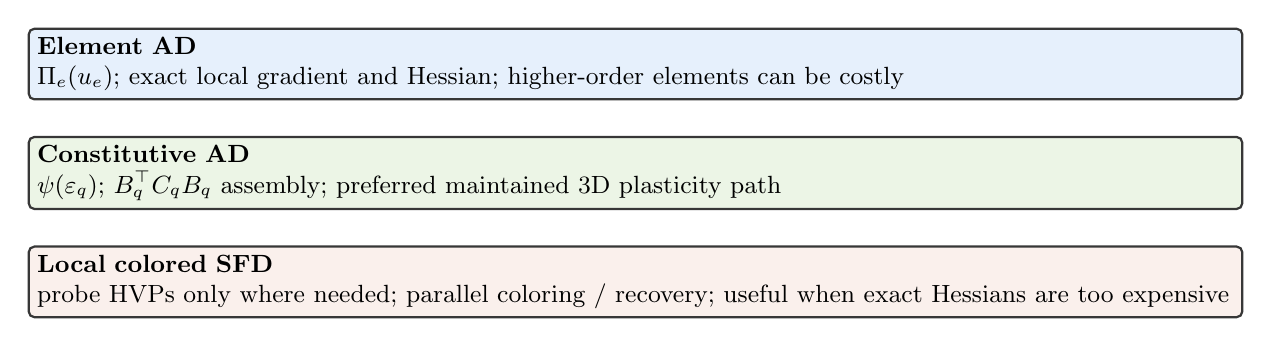
\begin{tikzpicture}[x=1cm,y=1cm]
  \node[paper box, fill=paperdiagblue, text width=15.2cm] (e) at (0,0)
    {\textbf{Element AD}\\$\Pi_e(u_e)$; exact local gradient and Hessian; higher-order elements can be costly};
  \node[paper box, fill=paperdiaggreen, text width=15.2cm, below=0.45cm of e] (c)
    {\textbf{Constitutive AD}\\$\psi(\varepsilon_q)$; $B_q^\top C_q B_q$ assembly; preferred maintained 3D plasticity path};
  \node[paper box, fill=paperdiagrose, text width=15.2cm, below=0.45cm of c] (s)
    {\textbf{Local colored SFD}\\probe HVPs only where needed; parallel coloring / recovery; useful when exact Hessians are too expensive};
\end{tikzpicture}%
}

\newcommand{\PaperGlobalizationDiagram}{%
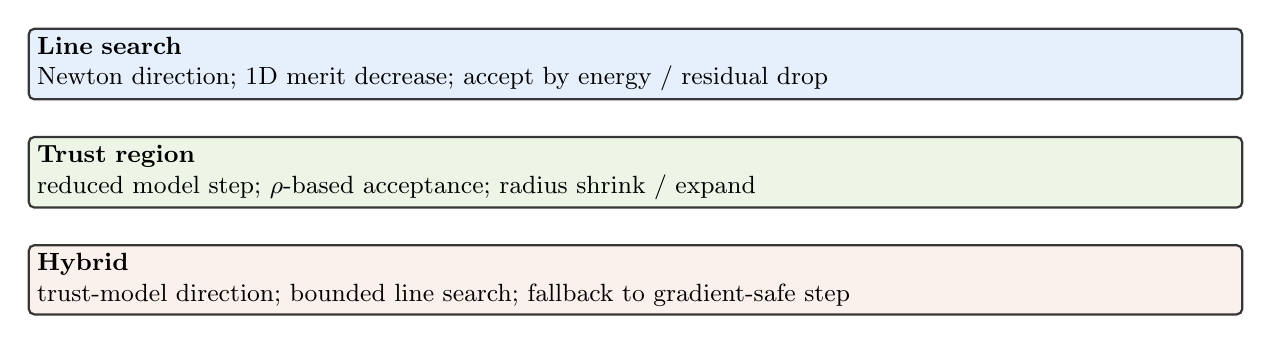
\begin{tikzpicture}[x=1cm,y=1cm]
  \node[paper box, fill=paperdiagblue, text width=15.2cm] (ls) at (0,0)
    {\textbf{Line search}\\Newton direction; 1D merit decrease; accept by energy / residual drop};
  \node[paper box, fill=paperdiaggreen, text width=15.2cm, below=0.45cm of ls] (tr)
    {\textbf{Trust region}\\reduced model step; $\rho$-based acceptance; radius shrink / expand};
  \node[paper box, fill=paperdiagrose, text width=15.2cm, below=0.45cm of tr] (hy)
    {\textbf{Hybrid}\\trust-model direction; bounded line search; fallback to gradient-safe step};
\end{tikzpicture}%
}

\newcommand{\PaperColoringDiagram}{%
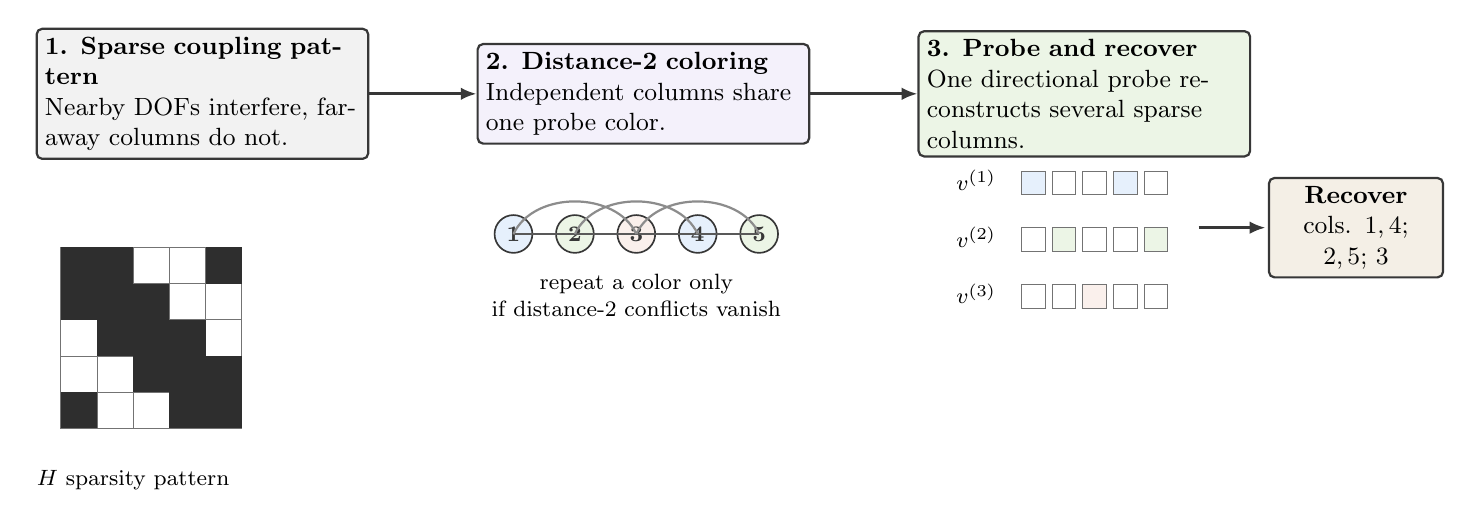
\begin{tikzpicture}[x=1cm,y=1cm]
  \tikzstyle{cell}=[draw=black!55, line width=0.30pt]
  \tikzstyle{stagearrow}=[paper arrow, line width=1.0pt]

  \node[paper box, fill=paperdiaggray, text width=4.0cm] (patternbox) at (0.0,0.0)
    {\textbf{1. Sparse coupling pattern}\\Nearby DOFs interfere, far-away columns do not.};
  \node[paper box, fill=paperdiagviolet, text width=4.0cm] (colorbox) at (5.6,0.0)
    {\textbf{2. Distance-2 coloring}\\Independent columns share one probe color.};
  \node[paper box, fill=paperdiaggreen, text width=4.0cm] (recoverbox) at (11.2,0.0)
    {\textbf{3. Probe and recover}\\One directional probe reconstructs several sparse columns.};

  \draw[stagearrow] (patternbox.east) -- (colorbox.west);
  \draw[stagearrow] (colorbox.east) -- (recoverbox.west);

  % Pattern panel
  \begin{scope}[shift={(-1.8,-1.95)}]
    \foreach \i in {0,...,4} {
      \foreach \j in {0,...,4} {
        \fill[white] (\i*0.46,-\j*0.46) rectangle ++(0.46,-0.46);
        \draw[cell] (\i*0.46,-\j*0.46) rectangle ++(0.46,-0.46);
      }
    }
    \foreach \i/\j in {
      0/0,1/0,0/1,1/1,
      1/2,2/1,2/2,2/3,3/2,3/3,
      3/4,4/3,4/4,
      0/4,4/0
    }{
      \fill[black!82] (\i*0.46,-\j*0.46) rectangle ++(0.46,-0.46);
    }
    \node[font=\footnotesize] at (0.92,-2.95) {$H$ sparsity pattern};
  \end{scope}

  % Coloring panel
  \begin{scope}[shift={(3.95,-1.78)}]
    \fill[paperdiagblue] (0.0,0) circle (0.24);
    \fill[paperdiaggreen] (0.78,0) circle (0.24);
    \fill[paperdiagrose] (1.56,0) circle (0.24);
    \fill[paperdiagblue] (2.34,0) circle (0.24);
    \fill[paperdiaggreen] (3.12,0) circle (0.24);
    \foreach \x/\lab in {0.0/1,0.78/2,1.56/3,2.34/4,3.12/5}{
      \draw[paperdiagdark,line width=0.6pt] (\x,0) circle (0.24);
      \node[font=\footnotesize\bfseries,text=paperdiagdark] at (\x,0) {\lab};
    }
    \draw[black!65,line width=0.8pt] (0.0,0) -- (0.78,0);
    \draw[black!65,line width=0.8pt] (0.78,0) -- (1.56,0);
    \draw[black!65,line width=0.8pt] (1.56,0) -- (2.34,0);
    \draw[black!65,line width=0.8pt] (2.34,0) -- (3.12,0);
    \draw[black!45,line width=0.8pt] (0.0,0) to[out=65,in=115] (1.56,0);
    \draw[black!45,line width=0.8pt] (0.78,0) to[out=65,in=115] (2.34,0);
    \draw[black!45,line width=0.8pt] (1.56,0) to[out=65,in=115] (3.12,0);
    \node[font=\footnotesize,align=center] at (1.56,-0.78) {repeat a color only\\if distance-2 conflicts vanish};
  \end{scope}

  % Recovery panel
  \begin{scope}[shift={(9.45,-2.08)}]
    \node[font=\footnotesize, anchor=west] at (0.00,0.98) {$v^{(1)}$};
    \node[font=\footnotesize, anchor=west] at (0.00,0.26) {$v^{(2)}$};
    \node[font=\footnotesize, anchor=west] at (0.00,-0.46) {$v^{(3)}$};
    \foreach \x in {0.95,1.34,1.73,2.12,2.51}{
      \fill[white] (\x,1.10) rectangle ++(0.30,-0.30);
      \draw[cell] (\x,1.10) rectangle ++(0.30,-0.30);
      \fill[white] (\x,0.38) rectangle ++(0.30,-0.30);
      \draw[cell] (\x,0.38) rectangle ++(0.30,-0.30);
      \fill[white] (\x,-0.34) rectangle ++(0.30,-0.30);
      \draw[cell] (\x,-0.34) rectangle ++(0.30,-0.30);
    }
    \fill[paperdiagblue] (0.95,1.10) rectangle ++(0.30,-0.30);
    \fill[paperdiagblue] (2.12,1.10) rectangle ++(0.30,-0.30);
    \fill[paperdiaggreen] (1.34,0.38) rectangle ++(0.30,-0.30);
    \fill[paperdiaggreen] (2.51,0.38) rectangle ++(0.30,-0.30);
    \fill[paperdiagrose] (1.73,-0.34) rectangle ++(0.30,-0.30);
    \draw[cell] (0.95,1.10) rectangle ++(0.30,-0.30);
    \draw[cell] (2.12,1.10) rectangle ++(0.30,-0.30);
    \draw[cell] (1.34,0.38) rectangle ++(0.30,-0.30);
    \draw[cell] (2.51,0.38) rectangle ++(0.30,-0.30);
    \draw[cell] (1.73,-0.34) rectangle ++(0.30,-0.30);
    \draw[stagearrow] (3.20,0.38) -- (4.05,0.38);
    \node[paper box, fill=paperdiagbeige, text width=2.0cm, align=center] at (5.2,0.38)
      {\textbf{Recover}\\cols. $1,4$;\\$2,5$; $3$};
  \end{scope}
\end{tikzpicture}%
}
